
\documentclass[oneside]{normas-utf-tex} %oneside = para dissertacoes com numero de paginas menor que 100 (apenas frente da folha) 

% force A4 paper format
%\special{papersize=210mm,297mm}

\usepackage[brazil]{babel} % pacote portugues brasileiro
\usepackage[utf8]{inputenc} % pacote para acentuacao direta
\usepackage{amsmath,amsfonts,amssymb} % pacote matematico
\usepackage{graphicx} % pacote grafico
%\usepackage{times} % fonte times
\usepackage[final]{pdfpages} % adicao da ata
\usepackage{hyperref} % gera hiperlinks para o sumario, links, referencias -- deve vir antes do 'abntcite' 
\usepackage{tabularx}
\usepackage{pgfgantt}
\usepackage{rotating}
\usepackage[alf,abnt-emphasize=bf,bibjustif,recuo=0cm, abnt-etal-cite=2, abnt-etal-list=99]{abntcite} %configuracao correta das referencias bibliograficas.
\usepackage{subfigure}
\usepackage{xtab}
\usepackage{nomencl}
%\usepackage[portuguese,algoruled,longend,linesnumbered]{algorithm2e} %Para linhas numeradas e réguas de identação
\usepackage{algorithm2e}
\usepackage{listings}
% Definindo novas cores
\definecolor{verde}{rgb}{0.25,0.5,0.35}
\definecolor{jpurple}{rgb}{0.5,0,0.35}
% Configurando layout para mostrar codigos Java
\lstset{
  language=Java,
  basicstyle=\ttfamily\small,
  keywordstyle=\color{jpurple}\bfseries,
  stringstyle=\color{red},
  commentstyle=\color{verde},
  morecomment=[s][\color{blue}]{/**}{*/},
  extendedchars=true,
  showspaces=false,
  showstringspaces=false,
  numbers=left,
  numberstyle=\tiny,
  breaklines=true,
  backgroundcolor=\color{cyan!10},
  breakautoindent=true,
  captionpos=b,
  xleftmargin=0pt,
  tabsize=4
}
\renewcommand{\lstlistingname}{Código}
\renewcommand\lstlistlistingname{Lista de Códigos}


% ---------- Preambulo ----------
\instituicao{Universidade Tecnol\'ogica Federal do Paran\'a} % nome da instituicao
\departamento{Departamento Acad\^{e}mico de Computa\c{c}\~ao} % nome do programa
\programa{Curso de Ci\^{e}ncia da Computa\c{c}\~ao} % área ou curso

\documento{Trabalho de Conclusão de Curso}
\nivel{Graduação}
\titulacao{Bacharel} 

\titulo{{Quadricóptero}} % titulo do trabalho em portugues
\title{\MakeUppercase{Quadrotor}} % titulo do trabalho em ingles

\autor{Fernando Padilha Ferreira} % autor do trabalho
\cita{FERREIRA, Fernando Padilha} % sobrenome (maiusculas), nome do autor do trabalho

\palavraschave{quadricóptero, multi-rotor, VTOL} % palavras-chave do trabalho
\keywords{quadrotor, multi-rotor, VTOL} % palavras-chave do trabalho em ingles

\comentario{\UTFPRdocumentodata\ apresentado ao \UTFPRdepartamentodata\ da \ABNTinstituicaodata\ como requisito parcial para obten\c{c}\~ao do título de ``\UTFPRtitulacaodata\ em Computação''.}

\orientador{Prof. Dr. Hugo Vieira Neto} % nome do orientador do trabalho

\primeiroassina{Prof. Fulano\\ UTFPR - Câmpus Medianeira}
\segundoassina{Prof. Fulano\\ UTFPR - Câmpus Medianeira}
\terceiroassina{Prof. Fulano\\ UTFPR - Câmpus Medianeira}
\quartoassina{Prof. Fulano\\ UTFPR - Câmpus Medianeira}
\textoaprovacao{Este \UTFPRdocumentodata\ foi apresentado \`{a}s xx:xxh do dia X de mês de 20XX como requisito parcial para a obtenção do título de \UTFPRtitulacaodata~no \UTFPRprogramadata, da \ABNTinstituicaodata, Câmpus Medianeira. O candidato foi arguido pela Banca Examinadora composta pelos professores abaixo assinados. Após deliberação, a Banca Examinadora considerou o trabalho aprovado.}

\local{Medianeira} % cidade
\data{\the\year} % ano automatico

% desativa hifenizacao mantendo o texto justificado.
% thanks to Emilio C. G. Wille
\tolerance=1
\emergencystretch=\maxdimen
\hyphenpenalty=10000
\hbadness=10000
\sloppy

\definecolor{laranjautfpr}{cmyk}{0.0, 0.2, 1.0, 0.0}
\usepackage{enumitem}
\setlist{leftmargin=2cm}
\setlist{nosep}


%---------- Inicio do Documento ----------
\begin{document}


\capa % geracao automatica da capa
\folhaderosto % geracao automatica da folha de rosto

\termodeaprovacao

%resumo
\begin{resumo}
Incluir o resumo aqui para testes de bla bla bla bla Incluir o resumo aqui para testes de bla bla bla bla Incluir o resumo aqui para testes de bla bla bla bla Incluir o resumo aqui para testes de bla bla bla bla Incluir o resumo aqui para testes de bla bla bla bla
\end{resumo}

%abstract
\begin{abstract}
Include the abstract here Include the abstract here Include the abstract here Include the abstract here Include the abstract here Include the abstract here Include the abstract here Include the abstract here Include the abstract here Include the abstract here.
\end{abstract}

%------------------------DEDICATÓRIA------------------------------

\begin{dedicatoria}
Dedicatória do trabalho (opcional). 
\end{dedicatoria}

%-----------------------AGRADECIMENTOS----------------------------
\begin{agradecimentos}
Agradecimentos do trabalho (opcional). 
\end{agradecimentos}
%-----------------------EPÍGRAFE-----------------------------------
\begin{epigrafe}
Epígrafe do trabalho (opcional). 
\end{epigrafe}



% listas (opcionais, mas recomenda-se a partir de 5 elementos)
\listadefiguras % geracao automatica da lista de figuras
\listadetabelas % geracao automatica da lista de tabelas
%\listadequadros % adivinhe :)
\listadesiglas % geracao automatica da lista de siglas
%\listadesimbolos % geracao automatica da lista de simbolos

% sumario
\sumario % geracao automatica do sumario


%---------- Inicio do Texto ----------
% recomenda-se a escrita de cada capitulo em um arquivo texto separado (exemplo: intro.tex, fund.tex, exper.tex, concl.tex, etc.) e a posterior inclusao dos mesmos no mestre do documento utilizando o comando \input{}, da seguinte forma:

%\setcounter{page}{48}

\setlength{\parskip}{0.0cm}
\chapter{Introdução}\label{ch:intro}

As aplicações dos Veículos Aéreos Não Tripulados (\sigla{VANT}{Veículos Aéreos Não Tripulados}s) há décadas atraem pesquisadores de diversas partes do mundo e tem gerado muitas pesquisas. Na última década, os avanços em materiais, componentes eletrônicos, sensores e baterias permitiram grandes avanços no desenvolvimento destes veículos. A utilização de VANTs permite retirar o ser humano de condições de alta periculosidade e permitir um maior grau de liberdade e flexibilidade, abrindo possibilidades em tarefas que seriam impraticáveis para um veículo tripulado.

Entre os diversos tipos de VANTs, os helicópteros tem grande destaque, em especial os elétricos. Classificados como \sigla{VTOL}{Vertical Take-Off and Landing} (do inglês, \textit{Vertical Take-Off and Landing}), eles se diferenciam pelas seguintes características: 1) possui alta capacidade de carga; 2) possui seis graus de liberdade\footnote{O helicóptero possui seis graus de liberdade: rotação e translação nos eixos X, Y e Z.}, que permite maior manobrabilidade; 3) capacidade de miniaturização; 4) precisam de pouco espaço para pouso e decolagem; e 5) podem ser utilizados em ambientes internos e externos. No entanto, apresentam menor autonomia de voo em relação a outros VANTs e são mais difíceis de controlar.

Além dos helicópteros convencionais, com um rotor principal e um auxiliar na cauda, existem os multi-rotores, com dois ou mais rotores principais. A topologia com quatro rotores, dispostos em forma de ``+'' ou de ``X'' em uma plataforma, chamada de quadricóptero, é uma das mais pesquisadas devido à sua simplicidade mecânica e à desafiadora tarefa de estabilização de voo.

O primeiro quadricóptero foi construído pelos irmãos Louis e Jaques Breguet, em 1907, época em que se desenvolviam os primeiros aviões e helicópteros \cite{leishman00}. Devido a falta de estabilidade e de meios de controle, ele só foi capaz de levantar voo por alguns segundos. Nas décadas seguintes outras iniciativas conseguiram grandes avanços, superando os helicópteros convencionais em tempo de voo, contudo, apresentando complexos meios de controle. Nos anos seguintes, avanços significativos ocorreram nos helicópteros e o quadricópteros foram rapidamente ultrapassados e esquecidos.

O interesse por quadricópteros só foi reaparecer em meados de 1993, agora como VANT, no projeto Hoverbot, da Universidade de Michigan \cite{borestein93}. Este, como outros projetos desenvolvidos na sequência, sofreu com dificuldades de estabilização e não foi bem sucedido. Em 2002, na Universidade da Pensilvânia, houve um dos primeiros casos de sucesso com o projeto de \citeonline{altug02}. Seguido de vários outros, como \cite{niceCU04}, \cite{starmac04} e \cite{bouabdallah07}, tratando da estabilização de voo. Esses avanços em grande parte foram possíveis devido aos avanços dos sensores \sigla{MEMS}{Micro-Electro-Mechanical Systems}.

Alguns projetos conseguiram ótimos resultados utilizando realimentação visual para estimar a posição do veículo, como é o caso das equipes do Laboratório GRASP, da Universidade da Pensilvânia, e da Flying Machine Arena, dos Institutos Federais de Tecnologia da Suíça. Suas capacidades incluem manobras em alta velocidade, apresentações musicais e captura de bolas em voo. No entanto, estes veículos não são autônomos e requerem um processamento externo \cite{Lupashin2010, michael2010}.

No Brasil poucos trabalhos foram publicados nesse tema. A dissertação de mestrado de \citeonline{melo2010}, da Universidade Federal do Espírito Santo, propõe um quadricóptero como plataforma para desenvolvimento de algoritmos de controle e em \citeonline{lopes2011}, o modelo matemático de um quadricóptero é utilizado para simular e avaliar técnicas de controle.

Na UTFPR, uma tentativa de construção de um quadricóptero foi realizada na disciplina Oficinas de Integração 2, do curso de Engenharia de Computação, por \citeonline{oficinas2}. Apesar de não bem sucedida, a iniciativa despertou o interesse local, a exemplo do prof. Hugo Vieira, que comprou os materiais necessários para construção em um projeto futuro. Esses materiais, gentilmente cedidos, agora serão utilizados na elaboração deste projeto.

Além das aplicações militares, de vigilância e busca e resgate, que incentivaram as pesquisas inicias nessa área, há uma grande ramo de aplicações dos quadricópteros para fins acadêmicos. Estes podem ser utilizados ensino de diversas áreas, como: algoritmos de controle, para estabilização; inteligência artificial, para detecção e desvio de obstáculos; processamento de imagens; sistemas multi-agentes, no estudo de comportamento coletivo; entre outras. Este projeto seria o primeiro passo para posterior utilização em outros projetos.


\section{Objetivos geral e específicos}

Esse trabalho tem como objetivo desenvolver um quadricóptero elétrico autônomo, capaz de voar a uma altura fixa e evitar colisões. Esse objetivo principal pode ser dividido nos seguintes objetivos específicos:

\begin{itemize}
\item projetar e montar a estrutura física;
\item modelar o sistema;
\item projetar e implementar o sistema de comunicação;
\item projetar e construir o sistema embarcado;
\item projetar e implementar o sistema de controle;
\item idealizar e conduzir experimentos reais de teste de navegação.
\end{itemize}


\section{Organização do documento}

Esse documento será organizado da seguinte forma. O Capítulo \ref{cap:funda} apresentará inicialmente uma breve história do desenvolvimento dos quadricópteros. Em seguida, são apresentados os trabalhos correlatos recentes, com o intuito de situar este trabalho no estágio atual do conhecimento. A metodologia utilizada se encontra no Capítulo \ref{cap:metod}, nele são descritas todas as etapas para o desenvolvimento do projeto. No Capítulo \ref{cap:recur} são listados os recursos de \textit{software} e \textit{hardware} utilizados, bem como a forma de aquisição de cada um. O estudo de viabilidade e um cronograma preliminar são apresentados no Capítulo \ref{cap:viabi} e, por fim, no Capítulo \ref{cap:concl} encontra-se a conclusão da proposta do trabalho de conclusão de curso.

\section{Exemplos gerais que podem ser usados no TCC}\label{subsec:ExemplosLatex}



\subsection{Titulo C}\label{ssubsec:tituloc}

.....Teste de citaç\~ao de autor: ~\cite{AikesJunior2011}. Podendo ser também \citeonline{AikesJunior2011}, dependendo do contexto.
.....Teste de referência de seç\~ao, cap\'itulo ou figura: Capítulo~\ref{ch:intro} = (Introduç\~ao), Figura~\ref{fig:tux_laplace} (Figura Tux), Tabela~\ref{tab:tab_exemplo} (Tabela).

Exemplo de Equação não numerada: $3 \times \sum_{i=0}^{j}\Delta$.

A Equação~\ref{eq:segundoGrau} é um exemplo de uma equação numerada:
\begin{equation}
x = \dfrac{-b \pm \sqrt{ \Delta}}{2 \times a}
\label{eq:segundoGrau}
\end{equation}


$3 \times 3$
$\boldmath{ 3 \times 3}$

Modelo de chamada de figura.

\begin{figure}[htb]
	\centering
	
\includegraphics[width=0.4\textwidth]{Imagens/tux_laplace.png} % <- formatos PNG, JPG e PDF
	\caption[Texto que vai aparecer na lista de fig.]{Texto que vai aparecer embaixo da imagem.}
\fonte{\cite{oge1999}}%citaç\~ao do livro onde pegou a figura	
	\label{fig:tux_laplace}
\end{figure}

Modelo de chamada de subfigures:
\begin{figure}[!htb]
\centering
\subfigure[]{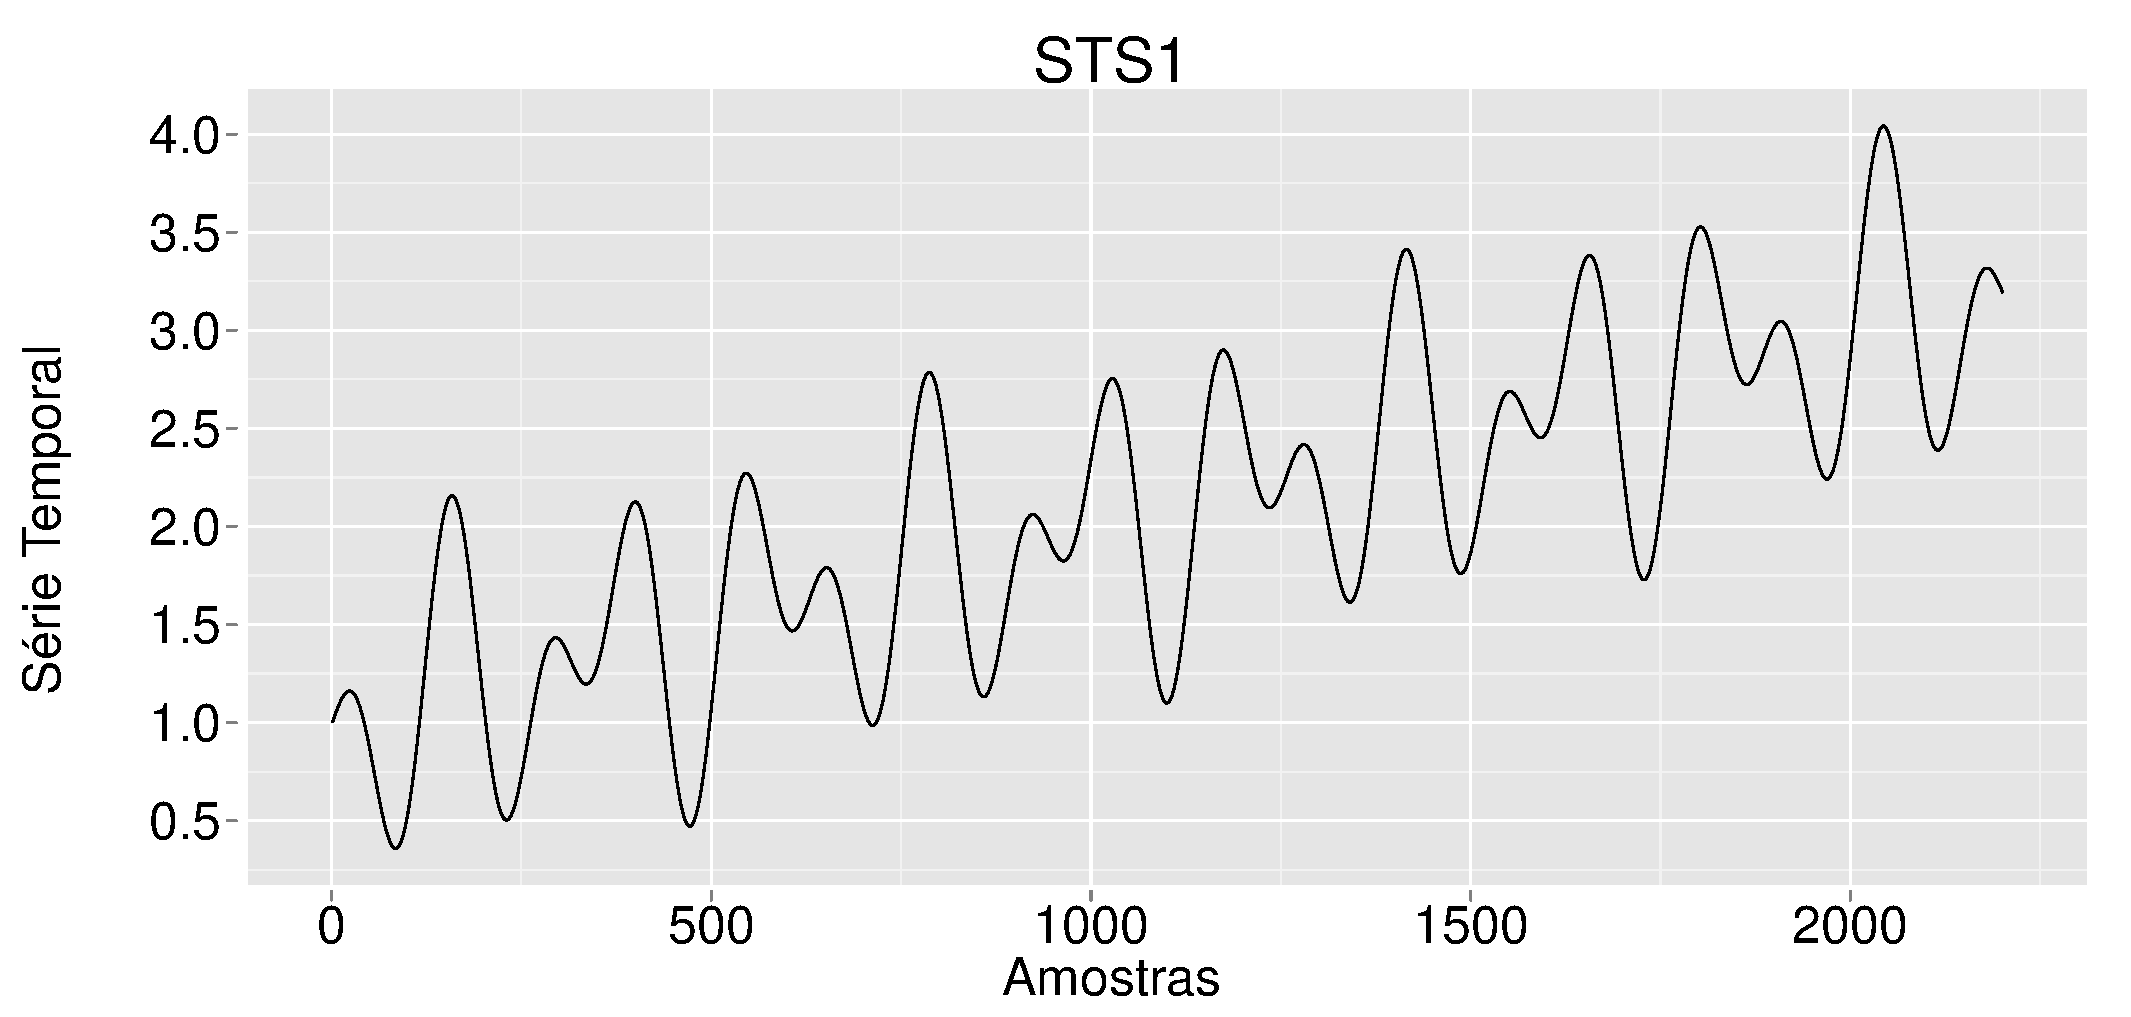
\includegraphics[width=0.49\textwidth]{Imagens/Arta1.pdf}}
\subfigure[]{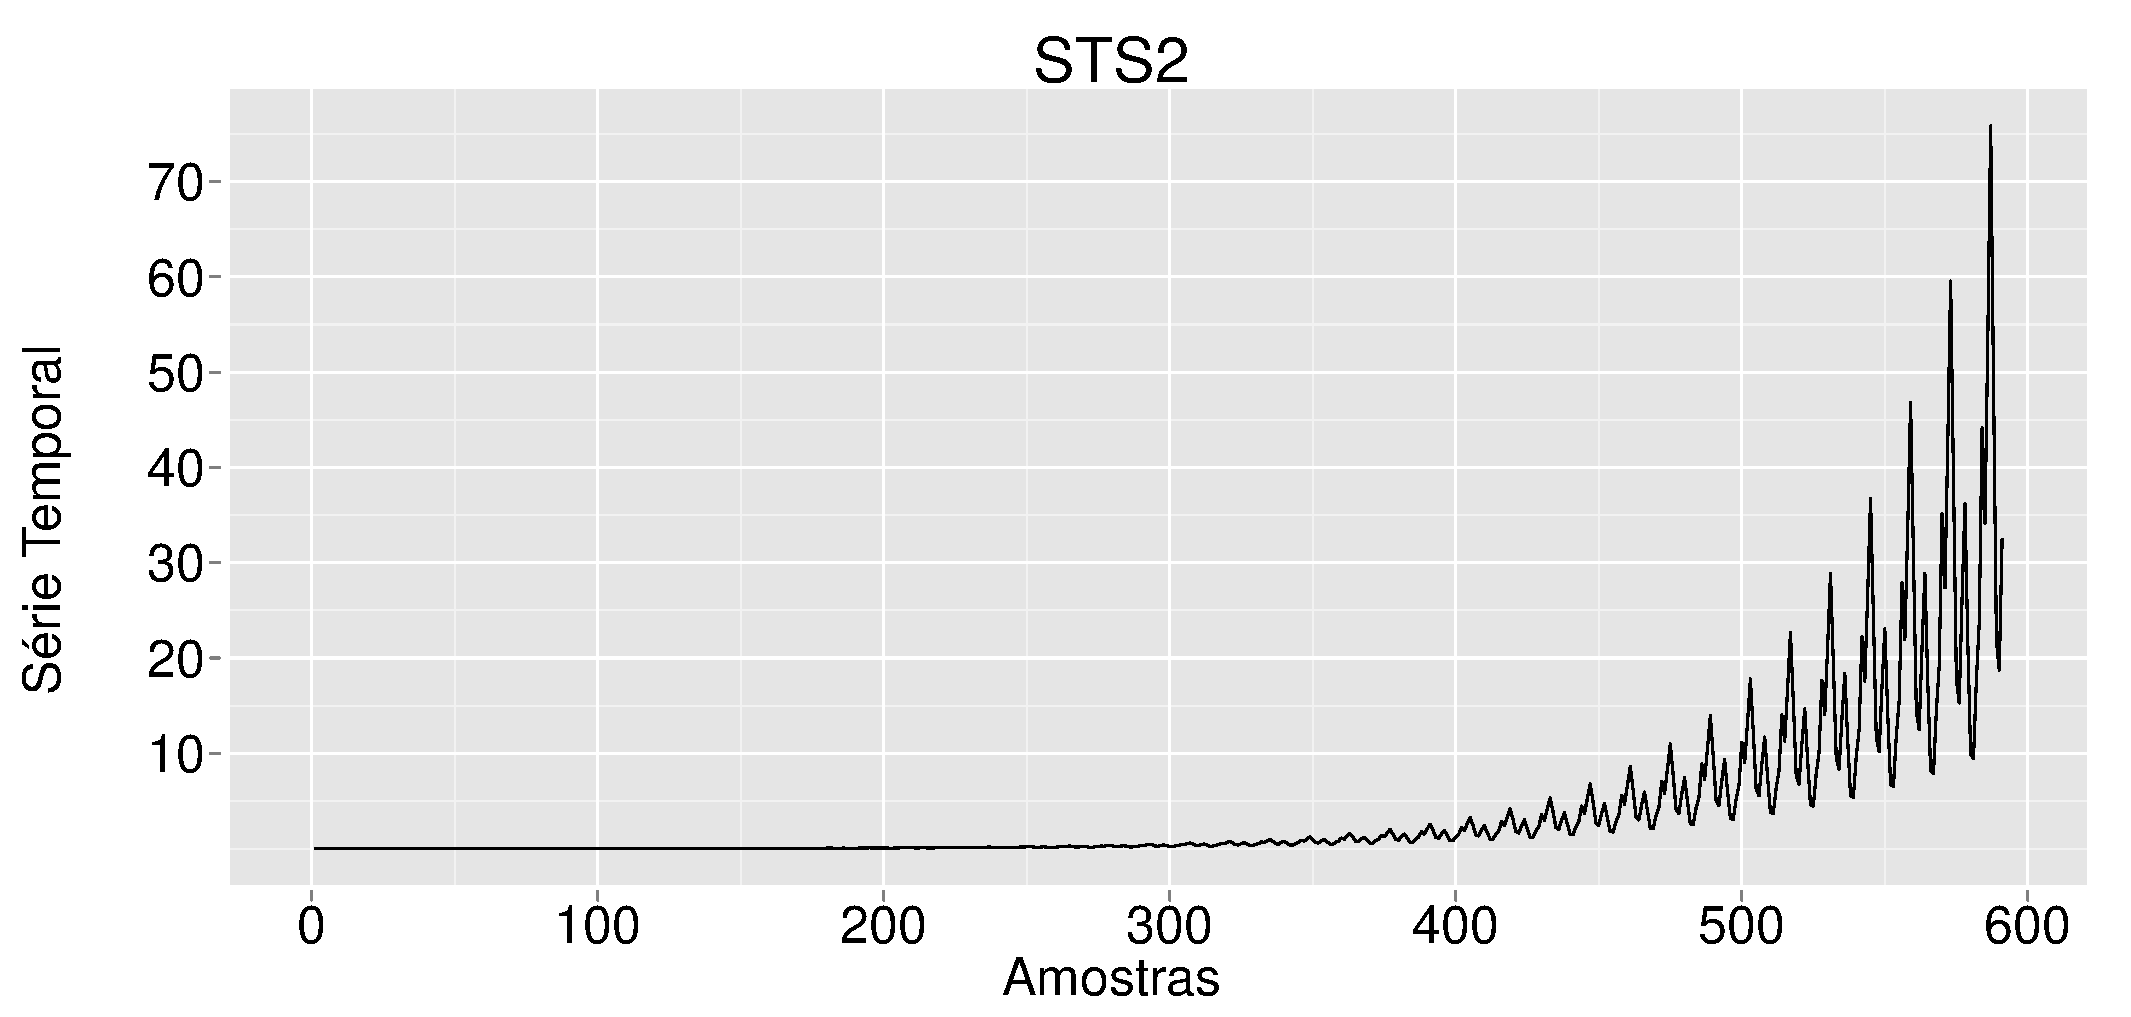
\includegraphics[width=0.49\textwidth]{Imagens/Arta2.pdf}}
\subfigure[]{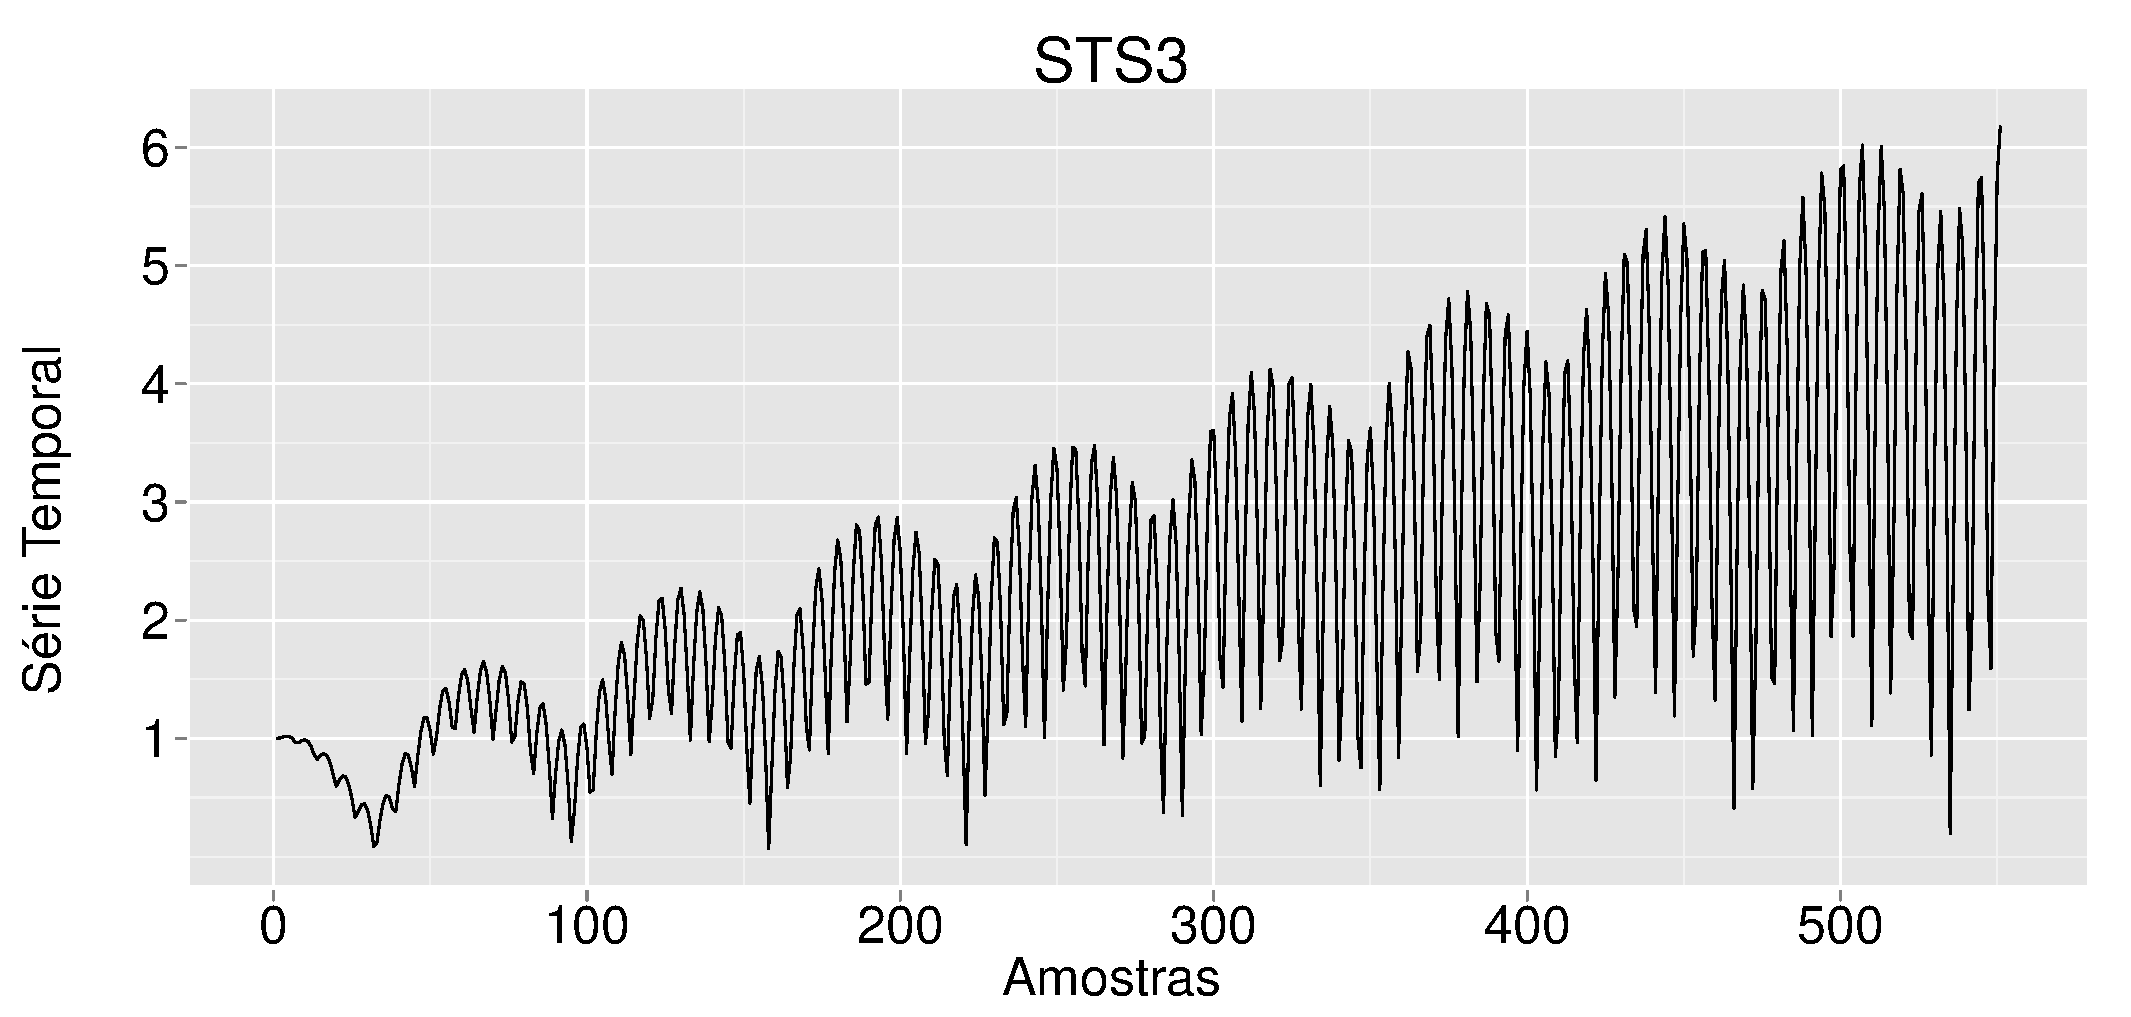
\includegraphics[width=0.49\textwidth]{Imagens/Arta3.pdf}}
\caption[Séries temporais artificiais geradas através de modelos sazonais]{Séries temporais artificiais geradas através de modelos sazonais: (a) STS1, (b) STS2 e (c) STS3.}
\label{fig:SeriesA}
\end{figure}


Modelo de tabela.
\begin{table}[!htb]
	\centering	
	\label{tab:tab_exemplo}
\begin{tabular}{|c|c|c|}
\hline 
Coluna 1 & Coluna 2 & Coluna 3 \\ 
\hline 
Conteúdo 1 & Conteúdo 2 & Conteúdo 3 \\ 
\hline 
\end{tabular} 
\caption[Texto da lista de tabelas]{Texto abaixo da tabela.}
\end{table}

Exemplo de algoritmo:
No Algoritmo~\ref{alg:kNNTSP}~\cite{Ferrero2009} é apresentado o pseudocódigo, em alto nível, do algoritmo, onde:
\begin{itemize}
\item $Z$ representa a ST utilizada;
\item $w$ representa o tamanho da janela para busca das sequências;
\item $M_s$ representa a medida de similaridade utilizada;
\item $C_k$ representa o critério utilizado para a seleção dos vizinhos próximos;
\item $k$ representa a quantidade de vizinhos mais próximos; e
\item $f$ representa a função de previsão utilizada para o cálculo do valor futuro.
\end{itemize}

\begin{algorithm}[hbtp]
\caption{\textit{$k$-NNTSP}.}
\label{alg:kNNTSP}
\Entrada{$Z$, $w$, $M_s$, $C_k$, $k$, $f$}
\Saida{$\hat{z}_{n+1};$}
\Inicio{
// Construção do conjunto de séries de treinamento $S$ a partir da série temporal $Z$ 

// e tamanho de janela $w$

$S \leftarrow series\_de\_treinamento(Z, w);$

// Definição da sequência de referência $U$

$U \leftarrow (z_n);$

// Obtenção das $k$ sequências mais próximas a $U$ contidas em $S$, considerando a

// medida de similaridade $M_s$ e o critério de seleção de vizinhos próximos $C_k$

$S' \leftarrow vizinhos\_proximos(S, U, M_s, C_k, k);$

// Cálculo do valor futuro da sequências de referências, utilizando $f(S')$

$\hat{z}_{n+1} \leftarrow f(S');$

\Retorna{$\hat{z}_{n+1}$}
}
\end{algorithm}

Exemplo de trecho de código.
\begin{lstlisting}[caption=Teste de Hello World]
/**
* comentario
*/
public class HelloWorldApp {
  public static void main (String argv[])
  {
    // Comentario
    System.out.println("Hello World!");
  }
}
\end{lstlisting}

Exemplo de tabela que ocupa mais de uma página (long tables):

\tablecaption{Características das ST disponíveis pela \textit{NNGC I}.} 
\tablefirsthead{\hline
    \hline
    \multicolumn{1}{c|}{{\scriptsize \textbf{Id}}} & \multicolumn{1}{c|}{{\scriptsize \textbf{Base de Dados}}} & \multicolumn{1}{c|}{{\scriptsize \textbf{Aquisição}}} & \multicolumn{1}{c|}{\scriptsize {\textbf{Tamanho}}} & \multicolumn{1}{c|}{{\scriptsize \textbf{Início }}} & \multicolumn{1}{c}{{\scriptsize \textbf{Término}}} \\
    \hline}
\tablehead{\multicolumn{6}{c}
    {{\tablename\ \thetable{ -- Características das ST disponíveis pela \textit{NNGC I}.}}} \\
    \hline 
    \hline
    \multicolumn{6}{r}
    {\scriptsize Continuação da página anterior.}\\
    \hline
    \multicolumn{1}{c|}{{\scriptsize \textbf{Id}}} & \multicolumn{1}{c|}{{\scriptsize \textbf{Base de Dados}}} & \multicolumn{1}{c|}{{\scriptsize \textbf{Aquisição}}} & \multicolumn{1}{c|}{\scriptsize {\textbf{Tamanho}}} & \multicolumn{1}{c|}{{\scriptsize \textbf{Início }}} & \multicolumn{1}{c}{{\scriptsize \textbf{Término}}}\\}
\tabletail{\hline 
\multicolumn{6}{r}
           {\scriptsize Continua na página seguinte.}\\
            }
\tablelasttail{\hline \hline}
%\xentrystretch{-0.15}
\begin{center}
\begin{xtabular}{c|c|c|c|c|c}
    {\scriptsize 1.B-001} & {\scriptsize 1.B}   & {\scriptsize Quaternal} & {\scriptsize 40}   & {\scriptsize jan-1993} & {\scriptsize abr-2002} \\ \hline
    {\scriptsize 1.B-002} & {\scriptsize 1.B}   & {\scriptsize Quaternal} & {\scriptsize 31}   & {\scriptsize jan-1990} & {\scriptsize mar-1997} \\ \hline
    {\scriptsize 1.B-003} & {\scriptsize 1.B}   & {\scriptsize Quaternal} & {\scriptsize 148}   & {\scriptsize jan-1967} & {\scriptsize abr-2003}\\ \hline
    {\scriptsize 1.B-004} & {\scriptsize 1.B}   & {\scriptsize Quaternal} & {\scriptsize 148}   & {\scriptsize jan-1967} & {\scriptsize abr-2003} \\ \hline
    {\scriptsize 1.B-005} & {\scriptsize 1.B}   & {\scriptsize Quaternal} & {\scriptsize 148}   & {\scriptsize jan-1967} & {\scriptsize abr-2003} \\ \hline
    {\scriptsize 1.B-006} & {\scriptsize 1.B}   & {\scriptsize Quaternal} & {\scriptsize 108}   & {\scriptsize jan-1977} & {\scriptsize abr-2003} \\ \hline
    {\scriptsize 1.B-007} & {\scriptsize 1.B}   & {\scriptsize Quaternal} & {\scriptsize 108}   & {\scriptsize jan-1977} & {\scriptsize abr-2003} \\ \hline
    {\scriptsize 1.B-008} & {\scriptsize 1.B}   & {\scriptsize Quaternal} & {\scriptsize 148}   & {\scriptsize jan-1967} & {\scriptsize abr-2003} \\ \hline
    {\scriptsize 1.B-009} & {\scriptsize 1.B}   & {\scriptsize Quaternal} & {\scriptsize 148}   & {\scriptsize jan-1967} & {\scriptsize abr-2003} \\ \hline
    {\scriptsize 1.B-010} & {\scriptsize 1.B}   & {\scriptsize Quaternal} & {\scriptsize 148}   & {\scriptsize jan-1967} & {\scriptsize abr-2003} \\ \hline
    {\scriptsize 1.B-011} & {\scriptsize 1.B}   & {\scriptsize Quaternal} & {\scriptsize 148}   & {\scriptsize jan-1967} & {\scriptsize abr-2003} \\ \hline
    {\scriptsize 1.C-001} & {\scriptsize 1.C}   & {\scriptsize Mensal} & {\scriptsize 48 }   & {\scriptsize jan-1999} & {\scriptsize dez-2002} \\ \hline
    {\scriptsize 1.C-002} & {\scriptsize 1.C}   & {\scriptsize Mensal} & {\scriptsize 48 }   & {\scriptsize jan-1999} & {\scriptsize dez-2002} \\ \hline
    {\scriptsize 1.C-003} & {\scriptsize 1.C}   & {\scriptsize Mensal} & {\scriptsize 198}   & {\scriptsize set-1987} & {\scriptsize fev-2004} \\ \hline
    {\scriptsize 1.C-004} & {\scriptsize 1.C}   & {\scriptsize Mensal} & {\scriptsize 172}   & {\scriptsize jan-1990} & {\scriptsize abr-2004} \\ \hline
    {\scriptsize 1.C-005} & {\scriptsize 1.C}   & {\scriptsize Mensal} & {\scriptsize 118}   & {\scriptsize out-1993} & {\scriptsize jul-2003} \\ \hline
    {\scriptsize 1.C-006} & {\scriptsize 1.C}   & {\scriptsize Mensal} & {\scriptsize 118}   & {\scriptsize out-1993} & {\scriptsize jul-2003} \\ \hline
    {\scriptsize 1.C-007} & {\scriptsize 1.C}   & {\scriptsize Mensal} & {\scriptsize 118}   & {\scriptsize out-1993} & {\scriptsize jul-2003} \\ \hline
    {\scriptsize 1.C-008} & {\scriptsize 1.C}   & {\scriptsize Mensal} & {\scriptsize 57 }   & {\scriptsize abr-1998} & {\scriptsize dez-2002} \\ \hline
    {\scriptsize 1.C-009} & {\scriptsize 1.C}   & {\scriptsize Mensal} & {\scriptsize 227}   & {\scriptsize jan-1983} & {\scriptsize nov-2001} \\ \hline
    {\scriptsize 1.C-010} & {\scriptsize 1.C}   & {\scriptsize Mensal} & {\scriptsize 132}   & {\scriptsize abr-1993} & {\scriptsize mar-2004} \\ \hline
    {\scriptsize 1.C-011} & {\scriptsize 1.C}   & {\scriptsize Mensal} & {\scriptsize 228}   & {\scriptsize mar-1986} & {\scriptsize fev-2005} \\ \hline
    {\scriptsize 1.D-001} & {\scriptsize 1.D}   & {\scriptsize Semanal} & {\scriptsize 527 }  & {\scriptsize 02-jan-1995} & {\scriptsize 31-jan-2005} \\ \hline
    {\scriptsize 1.D-003} & {\scriptsize 1.D}   & {\scriptsize Semanal} & {\scriptsize 437 }  & {\scriptsize 03-jan-1997} & {\scriptsize 13-mai-2005} \\ \hline
    {\scriptsize 1.D-004} & {\scriptsize 1.D}   & {\scriptsize Semanal} & {\scriptsize 549 }  & {\scriptsize 11-nov-1994} & {\scriptsize 13-mai-2005} \\ \hline
    {\scriptsize 1.D-005} & {\scriptsize 1.D}   & {\scriptsize Semanal} & {\scriptsize 437 }  & {\scriptsize 03-jan-1997} & {\scriptsize 13-mai-2005} \\ \hline
    {\scriptsize 1.D-006} & {\scriptsize 1.D}   & {\scriptsize Semanal} & {\scriptsize 618 }  & {\scriptsize 16-jul-1993} & {\scriptsize 13-mai-2005} \\ \hline
    {\scriptsize 1.D-007} & {\scriptsize 1.D}   & {\scriptsize Semanal} & {\scriptsize 618 }  & {\scriptsize 16-jul-1993} & {\scriptsize 13-mai-2005} \\ \hline
    {\scriptsize 1.D-008} & {\scriptsize 1.D}   & {\scriptsize Semanal} & {\scriptsize 548 }  & {\scriptsize 18-nov-1994} & {\scriptsize 13-mai-2005} \\ \hline
    {\scriptsize 1.D-009} & {\scriptsize 1.D}   & {\scriptsize Semanal} & {\scriptsize 548 }  & {\scriptsize 18-nov-1994} & {\scriptsize 13-mai-2005} \\ \hline
    {\scriptsize 1.D-010} & {\scriptsize 1.D}   & {\scriptsize Semanal} & {\scriptsize 593 }  & {\scriptsize 07-jan-1994} & {\scriptsize 13-mai-2005} \\ \hline
    {\scriptsize 1.D-011} & {\scriptsize 1.D}   & {\scriptsize Semanal} & {\scriptsize 594 }  & {\scriptsize 10-jan-1994} & {\scriptsize 23-mai-2005} \\ \hline
    {\scriptsize 1.E-001} & {\scriptsize 1.E}   & {\scriptsize Diária} & {\scriptsize 377}   & {\scriptsize 01-jan-2005} & {\scriptsize 12-jan-2006} \\ \hline
    {\scriptsize 1.E-002} & {\scriptsize 1.E}   & {\scriptsize Diária} & {\scriptsize 377}   & {\scriptsize 01-jan-2005} & {\scriptsize 12-jan-2006} \\ \hline
    {\scriptsize 1.E-004} & {\scriptsize 1.E}   & {\scriptsize Diária} & {\scriptsize 466}   & {\scriptsize 07-fev-2003} & {\scriptsize 17-mai-2004} \\ \hline
    {\scriptsize 1.E-005} & {\scriptsize 1.E}   & {\scriptsize Diária} & {\scriptsize 716}   & {\scriptsize 01-jan-2002} & {\scriptsize 17-dez-2003} \\ \hline
    {\scriptsize 1.E-006} & {\scriptsize 1.E}   & {\scriptsize Diária} & {\scriptsize 502}   & {\scriptsize 01-jan-2002} & {\scriptsize 17-mai-2003} \\ \hline
    {\scriptsize 1.E-007} & {\scriptsize 1.E}   & {\scriptsize Diária} & {\scriptsize 502}   & {\scriptsize 01-jan-2002} & {\scriptsize 17-mai-2003} \\ \hline
    {\scriptsize 1.E-008} & {\scriptsize 1.E}   & {\scriptsize Diária} & {\scriptsize 747}   & {\scriptsize 01-nov-2003} & {\scriptsize 16-nov-2005} \\ \hline
    {\scriptsize 1.E-009} & {\scriptsize 1.E}   & {\scriptsize Diária} & {\scriptsize 747}   & {\scriptsize 01-nov-2003} & {\scriptsize 16-nov-2005} \\ \hline
    {\scriptsize 1.E-010} & {\scriptsize 1.E}   & {\scriptsize Diária} & {\scriptsize 654}   & {\scriptsize 01-jul-2003} & {\scriptsize 14-abr-2005} \\ \hline
    {\scriptsize 1.E-011} & {\scriptsize 1.E}   & {\scriptsize Diária} & {\scriptsize 654}   & {\scriptsize 01-jul-2003} & {\scriptsize 14-abr-2005} \\ \hline
    {\scriptsize 1.F-003} & {\scriptsize 1.F}   & {\scriptsize Horária (5:00-24:00)} & {\scriptsize 1742}  & {\scriptsize 02-jan-2005} & {\scriptsize 29-mar-2005} \\ \hline
    {\scriptsize 1.F-004} & {\scriptsize 1.F}   & {\scriptsize Horária (5:00-24:00)} & {\scriptsize 902 }  & {\scriptsize 05-set-2005} & {\scriptsize 19-out-2005} \\ \hline
    {\scriptsize 1.F-005} & {\scriptsize 1.F}   & {\scriptsize Horária (5:00-24:00)} & {\scriptsize 902 }  & {\scriptsize 05-set-2005} & {\scriptsize 19-out-2005} \\ \hline
    {\scriptsize 1.F-006} & {\scriptsize 1.F}   & {\scriptsize Horária (5:00-24:00)} & {\scriptsize 1742}  & {\scriptsize 02-jan-2005} & {\scriptsize 29-mar-2005} \\ \hline
    {\scriptsize 1.F-007} & {\scriptsize 1.F}   & {\scriptsize Horária (5:00-24:00)} & {\scriptsize 1742}  & {\scriptsize 02-jan-2005} & {\scriptsize 29-mar-2005} \\ \hline
    {\scriptsize 1.F-008} & {\scriptsize 1.F}   & {\scriptsize Horária (5:00-24:00)} & {\scriptsize 1742}  & {\scriptsize 02-jan-2005} & {\scriptsize 29-mar-2005} \\ \hline
    {\scriptsize 1.F-009} & {\scriptsize 1.F}   & {\scriptsize Horária (5:00-24:00)} & {\scriptsize 902 }  & {\scriptsize 05-set-2005} & {\scriptsize 19-out-2005} \\ \hline
    {\scriptsize 1.F-010} & {\scriptsize 1.F}   & {\scriptsize Horária (5:00-24:00)} & {\scriptsize 902 }  & {\scriptsize 05-set-2005} & {\scriptsize 19-out-2005} \\ \hline
    {\scriptsize 1.F-011} & {\scriptsize 1.F}   & {\scriptsize Horária (5:00-24:00)} & {\scriptsize 902 }  & {\scriptsize 05-set-2005} & {\scriptsize 19-out-2005} \\ 
\end{xtabular}
\end{center}







\chapter{Levantamento Bibliográfico} \label{cap:funda}

Nessa seção será descrito o estado da arte do tema escolhido. Primeiramente será dado uma breve história do desenvolvimento dos quadricópteros e, em seguida, serão apresentados os trabalhos correlatos recentes.

\section{História dos quadricópteros}

O desenvolvimento dos primeiros quadricópteros começou a mais de um século. Em 1907, os irmãos franceses Louis e Jaques Breguet construíram o primeiro quadricóptero pilotado, chamado de \textit{Gyroplane nº 1} \cite{leishman00}. A estrutura era constituída por quatro vigas, formadas de tubos de aço, dispostas em formato de cruz e com um lugar para o piloto ao centro, próximo ao motor. No entanto, devido a falta de estabilidade e de meios de controle, ele só foi capaz de levantar voo por alguns segundos.

Nas décadas seguintes houve grandes avanços em desempenho e controle dos quadricópteros. Em 1922, G. de Bothezat, um imigrante russo nos Estados Unidos, conseguiu realizar vários voos a baixas altitudes e baixas velocidades. Em 1924, o francês E. Oehmichen recebeu um prêmio da \sigla{FAI}{Federação Aeronáutica Internacional} por demonstrar um voo do seu quadricóptero em um circuito fechado de 1 km, com duração de 7 minutos e 40 segundos. Foi o primeiro helicóptero conseguir percorrer essa distância. Ambos os projetos foram cancelados por serem impraticáveis para uso real e pelo alto custo de desenvolvimento.

Alguns anos depois, em 1956, nos Estados Unidos, o Convertawings Modelo A reviveu os projetos de Bothezat e Oehmichen \cite{lambermont58}. Inventado por D. H. Kaplan, esse quadricóptero tinha os quatro rotores posicionados em forma de ``H'', ao invés de ``+'', como nos anteriores. Apesar de ter sido testado com sucesso, o apoio do Exército dos EUA foi encerrado.

O interesse pelos quadricopteros caiu com o início da comercialização de helicópteros convencionais, de um ou dois rotores, e só foi retomado na década de 90, desta vez no contexto de VANTs.

\subsection{Teste de Terceiro Nível}

%
aaaa

\begin{figure}[htb]
	\centering
	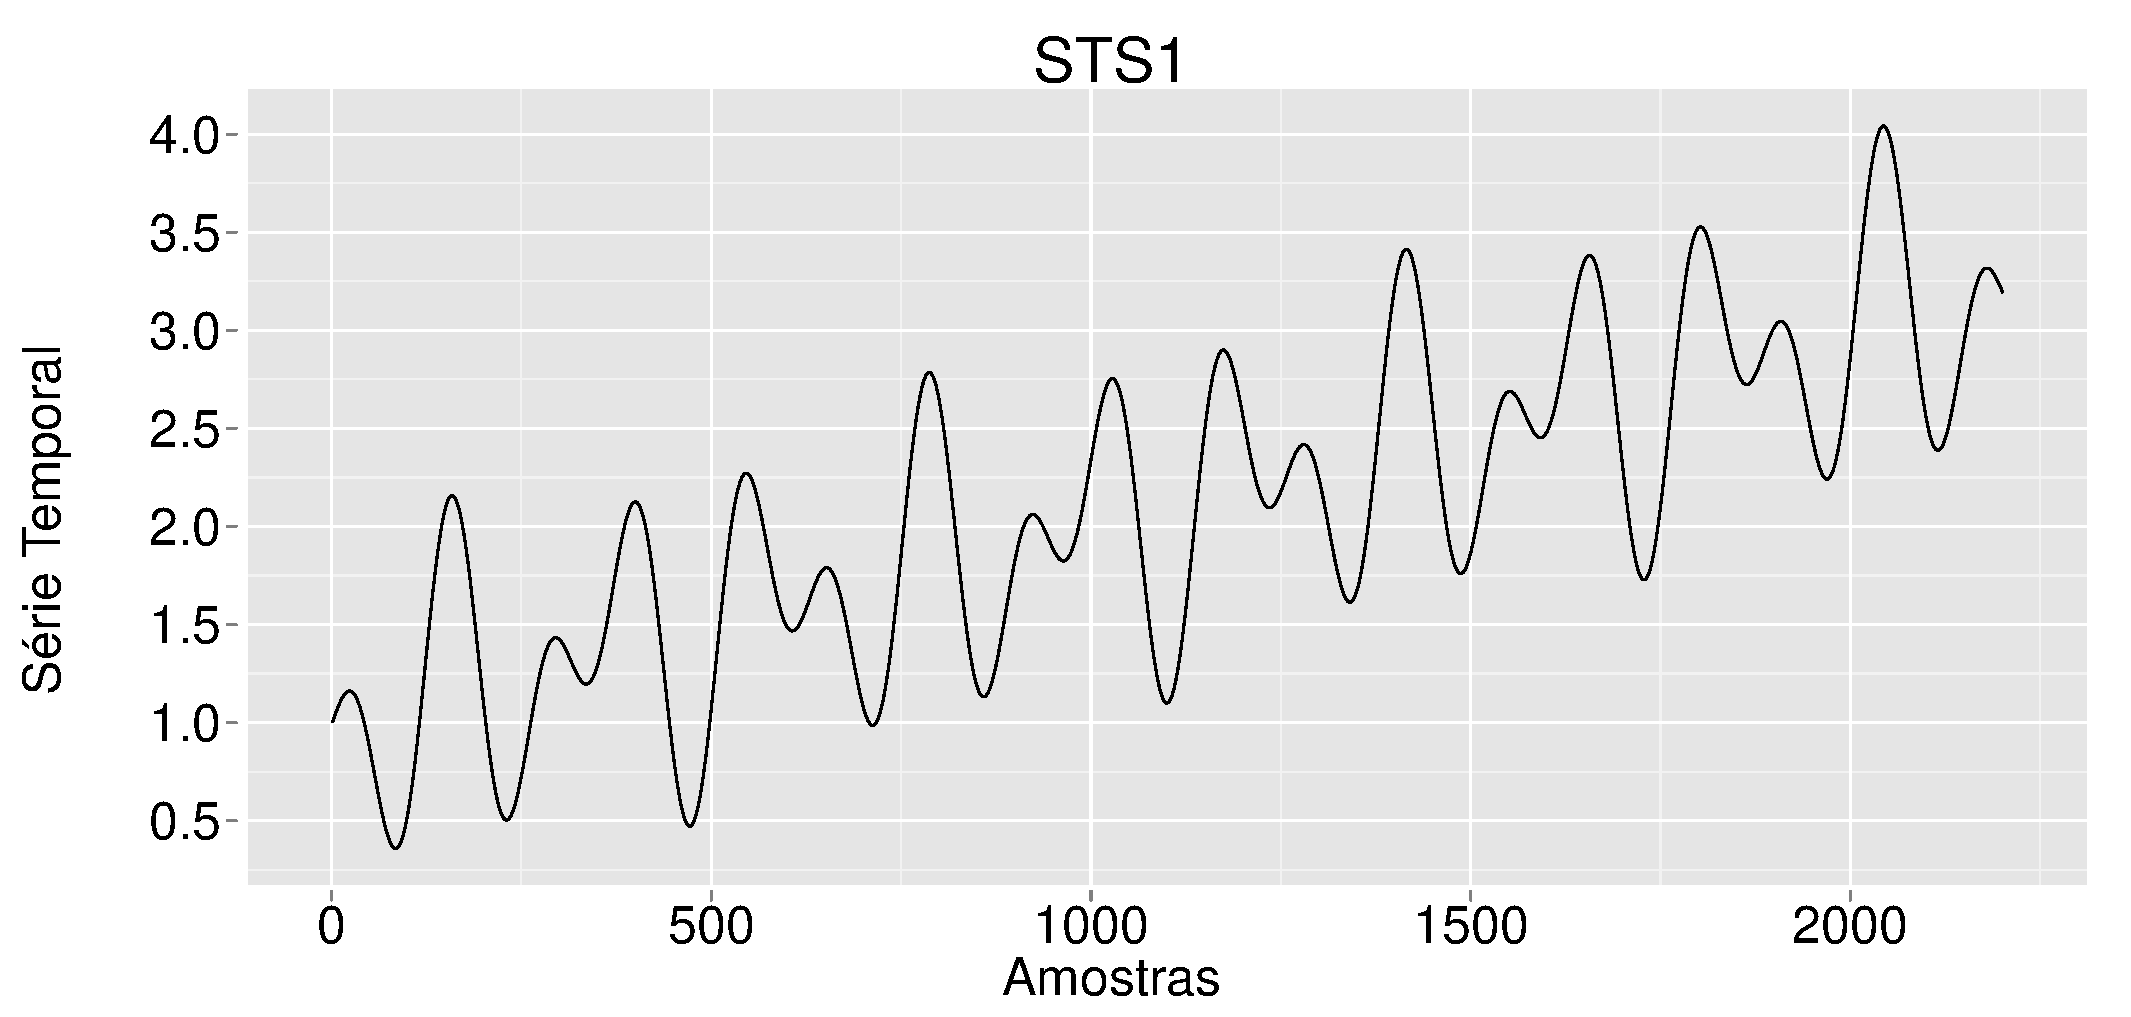
\includegraphics[width=0.4\textwidth]{Imagens/Arta1} % <- formatos PNG, JPG e PDF
	\caption[Texto que vai aparecer na lista de fig.]{Texto que vai aparecer embaixo da imagem.}
\fonte{\citeonline{AikesJunior2011}}%citaç\~ao do livro onde pegou a figura	
	\label{fig:tux_laplace}
\end{figure}

\section{Trabalhos correlatos}

Os desenvolvimentos recentes em materiais mais leves, componentes eletrônicos, motores elétricos, baterias e, principalmente, MEMS, permitiram que os VANTs se tornassem realidade. Com isso, muitos projetos de quadricópteros foram desenvolvidos independentemente 

Um dos primeiros projetos de quadricóptero VANT publicados foi o Hoverbot, em 1993 na Universidade de Michigan, construído basicamente pela união de quatro helicópteros de brinquedo pela cauda. O projeto foi rapidamente abandonado pelas dificuldades na construção do \textit{hardware}, mas conseguiu planar com o auxílio de uma estrutura que inibia seus movimentos horizontais \cite{borestein93}.

O projeto Mesicopter, desenvolvido em 2001 na Universidade de Stanford, buscava desenvolver quadricópteros na escala de centímetros e com massa de 3 a 15g. Sua aplicação seria para coleta de dados atmosféricos ou metereológicos em grandes áreas ou planetas. No entanto, ele nunca foi capaz de levantar o peso da sua fonte de alimentação \cite{kroo01}.

Em 2002, na Universidade da Pensilvânia, E. Altug desenvolveu um quadricóptero baseado em realimentação visual. O sistema de visão usa câmeras no solo para estimar a posição e a orientação, baseado em círculos coloridos dispostos no veículo, que servem de entrada para o sistema de controle, cuja saída é enviada ao quadricóptero. Duas técnicas de controle foram testadas: \textit{feedback linearization} e \textit{backstepping}. O veículo utilizado foi baseado no brinquedo HMX-4 \cite{altug02}.

Outro estudo foi a dissertação de mestrado de E. B. Nice, realizado em 2004 na Universidade de Cornell. Seu trabalho envolveu desenvolvimento completo da estrutura e controle. Foram utilizados um Filtro Sigma Point para estimar o estado e um controle LQR para estabilização. O veículo final pesava 6,2 kg. Durante os testes foi comprovada sua capacidade de planar a uma altura fixa, porém não foi possível completar os testes devido a falhas no \textit{hardware} \cite{niceCU04}. O projeto teve continuidade com o trabalho de Oliver Purwin, em 2009, no qual foi utilizado \textit{Iterative Learning Control} (\sigla{ILC}{Iterative Learning Control}, do inglês, controle por aprendizado iterativo) para realizar manobras agressivas \cite{purICRA09}. Desta vez não ocorreram problemas e os testes foram bem sucedidos.

Em 2003, no Instituto Federal de Tecnologia da Suíça , S. Bouabdallah começou o desenvolvimento de um quadricóptero chamado OS4. O projeto visava um sistemático processo de modelagem, desenvolvimento e controle de helicópteros miniatura, o qual foi aplicado no OS4. Foram testados cinco tipos de controladores: baseado na teoria de Lyapunov, \sigla{PID}{Proporcional Integral Derivativo} (Proporcional Integral Derivativo), \sigla{LQ}{Linear Quadrático} (Linear Quadrático), \textit{backstepping} e \textit{sliding-mode}. Por fim, foi escolhida a técnica de \textit{backstepping} incrementada com ação integral. O projeto teve sua conclusão em 2007, com a defesa da tese de doutorado de Bouabdallah \cite{bouabdallah07}. 

Em 2004, foi criado um projeto na Universidade de Stanford com o intuito de testar e validar algoritmos de controle multi-agentes, chamado de STARMAC. Alguns campos de estudo foram: detecção de obstáculos e colisão com outros veículos, formação de voo e seguir trajetória, usando técnicas centralizadas ou descentralizadas. Para seu controle foram utilizadas três técnicas: \textit{Integral Sliding Mode}, \textit{Reinforcement Learning} e filtros de Kalman. O quadricóptero utilizado era uma modificação do brinquedo Draganflyer III, foi um dos primeiros projetos a trabalhar em ambiente externo (\textit{outdoor}). O projeto teve continuidade com em 2007, o STARMAC II, com uma versão própria do quadricóptero e com melhorias no desempenho do controlador \cite{starmac04, starmac07}.

Outros dois projetos de grande interesse, com características bem semelhantes, mas desenvolvidos independentemente, são os projetos do Laboratório GRASP da Universidade da Pensilvânia e da Flying Machine Arena do Instituto Federal de Tecnologia da Suíça. Ambos utilizam versões modificadas do quadricóptero ``Hummingbird'', vendido pela Ascending Technologies, como também o sistema de captura de movimentos Vicon, que provê a posição do quadricóptero a uma taxa de 200 Hz e com precisão milimétrica \cite{Lupashin2010, michael2010}. Ao contrário da maioria trabalhos anteriores, esses veículos não são autônomos, eles dependem de um processamento externo para calcular seu próximo movimento, reduzindo o processamento embarcado. Apesar das limitações impostas pelo sistema de câmeras, a precisão obtida permitiu a realização de tarefas complexas, inalcançáveis até hoje com os quadricópteros autônomos .

Estão em desenvolvimento novas alternativas para navegação autônoma baseadas no mapeamento em 3D do ambiente. As abordagens incluem o uso de scanners a LASER \cite{dryanovski11}, sensores Microsoft Kinect \cite{stowers11} ou ambos \cite{shen12}.

No Brasil poucos trabalhos foram publicados nesse tema. A dissertação de mestrado de \citeonline{melo2010}, da Universidade Federal do Espírito Santo, propõe um quadricóptero como plataforma para desenvolvimento de algoritmos de controle. Ele descreve os componentes utilizados, as placas microcontroladas desenvolvidas e a do software sistema embarcado implementação, fazendo a interface com o rádio, os sensores e os motores e deixando livre a implementação do algoritmo de controle. São realizados testes de comunicação, leitura dos sensores e ativação dos motores, mas nenhum algoritmo de controle é testado para validar o funcionamento completo veículo. Em \citeonline{lopes2011}, o modelo matemático de um quadricóptero é utilizado para simular e avaliar técnicas de controle. É proposto o uso de um único controlador \textit{Model Predictive Control} (\sigla{MPC}{Model Predictive Control}) para controlar posição e estabilidade do sistema, ao ínves de dois controladores separados, como visto na literatura. Os resultados são comparados com controladores PID e \textit{backstepping}, mostrando-se melhor que o primeiro e inferior ao segundo.
\chapter{Metodologia} \label{cap:metod}

Nesse capítulo será descrita a metodologia utilizada para o desenvolvimento deste projeto. Serão descritas as etapas do projeto e os principais fundamentos e tecnologias a serem empregados.

O trabalho será composto por seis etapas:

\begin{enumerate}
\item Projetar e montar a estrutura física.
\item Modelar o sistema.
\item Projetar e implementar o sistema de comunicação.
\item Projetar e construir o sistema embarcado.
\item Projetar e implementar o sistema de controle.
\item Idealizar e conduzir experimentos reais de teste de navegação.
\end{enumerate}

\noindent{\bf Etapa 1:} essa etapa será destinada ao projeto, aquisição e montagem da estrutura física do quadricóptero. A estrutura é composta basicamente por um chassi, quatro motores, quatro hélices e uma bateria. Deverão ser analisados os recursos disponíveis no mercado ou passíveis de empréstimo capazes de satisfazer os requisitos do sistema. Ao final desta etapa, a estrutura deverá ser testada com o sistema eletrônico de um quadricóptero de controle remoto comercial, a fim de verificar suas capacidades básicas de voo.

\noindent{\bf Etapa 2:} nessa fase será feita a modelagem matemática da estrutura física desenvolvida na etapa anterior. Essa modelagem é necessária para o projeto do sistema de controle que será desenvolvido na etapa 5. Apesar de ter um grande foco teórico, também serão necessários testes empíricos.

\noindent{\bf Etapa 3:} aqui deverá ser desenvolvido o sistema de comunicação. Haverá dois canais de comunicação: um principal (quadricóptero-estação base), para definição de objetivos e coleta de dados, e um secundário (quadricóptero-controle remoto), de emergência, para que um humano possa assumir o controle. Deverão ser analisadas as tecnologias disponíveis, custo de implementação e integração com o sistema embarcado, a estação base e o controle remoto.

\noindent{\bf Etapa 4:} essa etapa é destinada o projeto e construção de um sistema embarcado microcontrolado para realização das funções do quadricóptero. O sistema deve ser capaz de realizar todas as tarefas em tempo real e de forma autônoma. Suas tarefas incluem: leitura dos sensores, comunicação, execução do sistema de controle de estabilidade e acionamento dos motores. Pode ser escolhido um sistema comercial, desde que atenda ao requisitos e que ofereça total acesso ao microcontrolador, ou pode ser desenvolvido um.

%O canal principal será entre o quadricóptero e uma estação base. A estação base enviará rotas de voo ou objetivos para o quadricóptero, e coletará dados dos sensores e estados internos. O canal secundário, ou de emergência, será estabelecido entre um controle remoto e o quadricóptero. Sua função é permitir que, em casos de mal funcionamento, risco de dano ao veículo ou a pessoas ao redor, um piloto externo possa assumir o controle e aterrissá-lo em uma posição segura.

\noindent{\bf Etapa 5:} nessa fase deverá ser projetado e implementado um sistema de controle de estabilidade e desvio de obstáculos. Diversas técnicas de controle já foram analisadas em outros projetos, cada uma apresentando vantagens e desvantagens, de acordo com as características do ambiente de estudo. Com base nesses trabalhos deverão ser escolhidas uma ou mais técnicas para utilização. Baseado na modelagem matemática desenvolvida na etapa 2, softwares matemáticos poderão ser utilizados para auxiliar no projeto do controlador, realizando simulações do funcionamento do sistema antes da implementação no sistema embarcado. Testes reais deverão ser realizados.

\noindent{\bf Etapa 6:} por fim, deverão ser conduzidos testes para verificar o funcionamento completo do veículo e validar os objetivos deste projeto.
\chapter{Recursos de Hardware e Software} \label{cap:recur}

Neste capítulo serão apresentados os principais recursos de \textit{hardware} e \textit{software} utilizados nesse projeto, bem como a origem destes recursos.


\section{Recursos de Hardware} \label{sec:recurhard}

Os recursos de \textit{hardware} necessários englobam o quadricóptero, o sistema de comunicação e a estação base.

O quadricóptero pode ser divido em duas partes: estrutura física e placa de controle. Os componentes da estrutura física são:

\begin{itemize}
\item 1x Chassi de 45cm diâmetro 
\item 4x Motor brushless 5000kV 
\item 4x Hélice 9x4,7 GWS 
\item 4x \sigla{ESC}{Eletronic Speed Control} 30A 
\item 1x Bateria 4000mAh 7,4V
\end{itemize}

estes componentes foram emprestados pelo prof. Hugo Vieira, orientador desse trabalho. Também foi emprestada uma placa de controle, chamada ``KK multicopter'', porém essa é uma placa de baixo desempenho e espera-se substituí-la por uma melhor. O desejável seria construir a própria placa de controle, porém devido ao encapsulamento \sigla{SMD}{Surface Mounted Device} utilizado nos sensores MEMS, a montagem dessas placas requer o uso de equipamentos específicos, inviáveis para esse projeto.

Até o momento não há disponibilidade de nenhum dos componentes do sistema de comunicação, todos deverão ser adquiridos. Eles são:

\begin{itemize}
\item 2x Módulo transceptor de RF
\item 1x USB \textit{dongle}
\item 1x Rádio controle 4 ou mais canais
\item 1x Receptor 4 ou mais canais
\end{itemize}

A estação base é um computador, desktop ou portátil, recente, com sistema operacional Windows ou Linux. Será usado um computador próprio.


\section{Recursos de Software}

Alguns recursos de software utilizados dependerão das alternativas de hardware escolhidas e só poderão ser definidas posteriormente. Inicialmente serão utilizados os seguintes:

\begin{itemize}
\item Matlab ou Octave: simulações do sistema de controle, coleta de dados do quadricóptero. Disponíveis na UTFPR e gratuito, respectivamente.
\item Eagle: criação de diagramas eletrônicos e placas de circuito impresso. Gratuito.
\item Astah community ou Dia: edição de diagramas UML e fluxogramas. Ambos gratuitos.
\end{itemize}








\chapter{Viabilidade e Cronograma Preliminar} \label{cap:viabi}

Neste capítulo será avaliada a viabilidade do projeto e será apresentado um cronograma preliminar de desenvolvimento.


\section{Viabilidade}

Como descrito no capítulo anterior, os principais recursos para a elaboração do projeto foram emprestados, para os de hardware, ou são gratuitos, para os de software. Resta para aquisição apenas os componentes da comunicação e da placa controladora. O gasto estimado para aquisição dos componentes e conclusão do projeto é de 300 reais, contanto que não ocorram danos no desenvolvimento, o que é completamente viável.


\section{Cronograma Preliminar}

A Tabela \ref{tab:crono} apresenta um cronograma preliminar do desenvolvimento do \sigla{TCC}{Trabalho de Conclusão de Curso}. Na sua elaboração foi considerado que o autor continuará o desenvolvimento no semestre seguinte, junto com a disciplina de TCC 2.

\begin{table}[!htb]
\caption{Cronograma} \label{tab:crono}
\begin{center}
	\begin{tabularx}{\textwidth}{|X|c|c|}
	\hline
	\textbf{Etapa} & \textbf{Data de início} & \textbf{Data de término} \\
	\hline
	Elaboração da proposta de TCC &
	11/12/12 & 19/03/13 \\
	\hline
	Entrega da proposta de TCC &
	26/03/13 & 26/03/13 \\
	\hline
	Elaboração do plano de projeto de TCC &
	26/04/13 & 23/04/13 \\
	\hline
	Entrega do plano de projeto de TCC &
	08/05/13 & 08/05/13 \\
	\hline
	Elaboração da monografia de TCC &
	03/06/13 & 10/10/13 \\
	\hline
	Projetar e montar a estrutura física &
	03/06/13 & 16/06/13 \\
	\hline
	Modelar o sistema &
	17/06/13 & 30/06/13 \\
	\hline
	Projetar e implementar o sistema de comunicação &
	01/07/13 & 28/07/13 \\
	\hline
	Projetar e construir o sistema embarcado &
	01/07/13 & 28/07/13 \\
	\hline
	Projetar e implementar o sistema de controle &
	29/07/13 & 01/09/13 \\
	\hline
	Idealizar e conduzir experimentos reais de teste de navegação &
	02/09/13 & 06/10/13 \\
	\hline
	Entrega da monografia e  defesa do TCC &
	11/10/13 & 11/10/13 \\
	\hline	
	\end{tabularx}
\end{center}
\end{table}

\chapter{Conclusões} \label{cap:concl}

Neste documento foi mostrada a viabilidade desse projeto para um trabalho de conclusão de curso. Este seria apenas o primeiro passo de uma série de outros projetos que poderiam aproveitar dos resultados obtidos. Há um grande ramo de aplicações para quadricópteros, como no estudo de algoritmos de controle, para estabilização; inteligência artificial, para detecção e desvio de obstáculos; processamento de imagens; sistemas multi-agentes, no estudo de comportamento coletivo; entre outros. Espera-se que, num futuro próximo, muitas outras surjam com os avanços tecnológicos, permitindo um maior tempo de voo e a realização de mais atividades de modo autônomo.


%---------- Referencias ----------
\clearpage % this is need for add +1 to pageref of bibstart used in 'ficha catalografica'.
\label{bibstart}
\bibliography{bibliografia} % geracao automatica das referencias a partir do arquivo bibliografia.bib
\label{bibend}



% --------- Ordenacao Afabetica da Lista de siglas --------
%\textbf{* Observa\c{c}\~oes:} a ordenacao alfabetica da lista de siglas ainda nao eh realizada de forma automatica, porem
% eh possivel se de realizar isto manualmente. Duas formas:
%
% ** Primeira forma)
%    A ordenacao eh feita com o auxilio do comando 'sort', disponivel em qualquer
% sistema Linux e UNIX, e tambem em sistemas Windows se instalado o coreutils (http://gnuwin32.sourceforge.net/packages/coreutils.htm)
% comandos para compilar e ordenar, supondo que seu arquivo se chame 'dissertacao.tex':
%
%      $ latex dissertacao
%      $ bibtex dissertacao && latex dissertacao
%      $ latex dissertacao
%      $ sort dissertacao.lsg > dissertacao.lsg.tmp
%      $ mv dissertacao.lsg.tmp dissertacao.lsg
%      $ latex dissertacao
%      $ dvipdf dissertacao.dvi
%
%
% ** Segunda forma)
%\textbf{Sugest\~ao:} crie outro arquivo .tex para siglas e utilize o comando \sigla{sigla}{descri\c{c}\~ao}.
%Para incluir este arquivo no final do arquivo, utilize o comando \input{arquivo.tex}.
%Assim, Todas as siglas serao geradas na ultima pagina. Entao, devera excluir a ultima pagina da versao final do arquivo
% PDF do seu documento.


%-------- Citacoes ---------
% - Utilize o comando \citeonline{...} para citacoes com o seguinte formato: Autor et al. (2011).
% Este tipo de formato eh utilizado no comeco do paragrafo. P.ex.: \citeonline{autor2011}

% - Utilize o comando \cite{...} para citacoeses no meio ou final do paragrafo. P.ex.: \cite{autor2011}



%-------- Titulos com nomes cientificos (titulo, capitulos e secoes) ----------
% Regra para escrita de nomes cientificos:
% Os nomes devem ser escritos em italico, 
%a primeira letra do primeiro nome deve ser em maiusculo e o restante em minusculo (inclusive a primeira letra do segundo nome).
% VEJA os exemplos abaixo.
% 
% 1) voce nao quer que a secao fique com uppercase (caixa alta) automaticamente:
%\section[nouppercase]{\MakeUppercase{Estudo dos efeitos da radiacao ultravioleta C e TFD em celulas de} {\textit{Saccharomyces boulardii}}
%
% 2) por padrao os cases (maiusculas/minuscula) sao ajustados automaticamente, voce nao precisa usar makeuppercase e afins.
% \section{Introducao} % a introducao sera posta no texto como INTRODUCAO, automaticamente, como a norma indica.


\end{document}
